\documentclass[a4paper,10pt]{article}
\usepackage[utf8]{inputenc}

\usepackage[english]{babel}
\usepackage[dvinames]{xcolor}
\usepackage[compact,small]{titlesec}
\usepackage{booktabs}
\usepackage{multirow}
\usepackage{amsfonts,amsmath,amssymb}
\usepackage{marginnote}
\usepackage[top=1.8cm, bottom=1.8cm, outer=1.8cm, inner=1.8cm, heightrounded, marginparwidth=2.5cm, marginparsep=0.5cm]{geometry}
\usepackage{enumitem}
\setlist{noitemsep,parsep=2pt}
\newcommand{\highlight}[1]{\textcolor{kuleuven}{#1}}
\usepackage{pythonhighlight}
\usepackage{cleveref}
\usepackage{graphicx}

\usepackage{float}
\usepackage{subcaption}
\usepackage{siunitx}

\newcommand{\nextyear}{\advance\year by 1 \the\year\advance\year by -1}
\newcommand{\thisyear}{\the\year}
\newcommand{\deadlineGroup}{November 27, \thisyear{} at 16:00 CET}
\newcommand{\deadlineCode}{December 18, \thisyear{} at 16:00 CET}
\newcommand{\deadlineReport}{January 4, \nextyear{} at 16:00 CET}

\newcommand{\ReplaceMe}[1]{{\color{blue}#1}}
\newcommand{\RemoveMe}[1]{{\color{purple}#1}}

\setlength{\parskip}{5pt}



%opening
\title{Evolutionary Algorithms: Final report}
\author{Simon Perneel}

\begin{document}
\fontfamily{ppl}
\selectfont{} 
\setlength\parindent{0pt} % no indentation

\maketitle

% \section{\RemoveMe{Formal requirements}} \label{sec_this}

% \RemoveMe{The report is structured for fair and efficient grading of over 100 individual projects in the space of only a few days. Please respect the exact structure of this document. You are allowed to remove sections \ref{sec_this} and \ref{sec_other}. Brevity is the soul of wit: a good report will be \textbf{around $7$ pages} long. The hard limit is 10 pages. 

% It is recommended that you use this \LaTeX{} template, but you are allowed to reproduce it with the same structure in a WYSIWYG-editor. The purple text containing our evaluation criteria can be removed. You should replace the blue text with your discussion. \textbf{The questions we ask in blue are there to guide which topics to discuss}, rather than an exact list of questions that must be answered. Feel free to add more items to discuss.

% This report should be uploaded to Toledo by \deadlineReport. It must be in the \textbf{Portable Document Format} (pdf) and must be named \texttt{r0123456\_final.pdf}, where r0123456 should be replaced with your student number.}

\section{Metadata}

\begin{itemize}
 \item \textbf{Group members during group phase:} Thomas Feys \& Timo Martens
 \item \textbf{Time spent on group phase:} 10 hours
 \item \textbf{Time spent on final code:} 42 hours
 \item \textbf{Time spent on final report:} 12 hours
\end{itemize}

\section{Modifications since the group phase}

% \RemoveMe{\textbf{Goal:} Based on this section, we will evaluate insofar as you are able to analyse common problems arising in the design and implementation of evolutionary algorithms and your ability to effectively solve them.}

\subsection{Main improvements}

% \ReplaceMe{List the main changes that you implemented since the group phase. You do not need to explain the employed techniques in detail; for this, you should refer to the appropriate subsection of section 3 of the report.}
The following paragraphs briefly describe the main improvements since the group phase. A more detailed explanation is given in section~\ref{sec:design}.

% \paragraph{Short description 1:} \ReplaceMe{State what modification you made (e.g., replaced top-$\lambda$ selection with $k$-tournament selection). What aspect of your evolutionary algorithm did it improve?} 

\paragraph{Initialization of the population:} The population is initialized now with an amount of heuristic good individuals. It leads the search into more promising areas of the search space and speeds up the optimization process. See section~\ref{ssec:initialization}~and~\ref{ssec:localsearch}.
\paragraph{More and better mutation operators:} In addition to swap mutation, insert mutation, scramble mutation and reverse sequence mutation has been implemented in order to increase randomness in the search. It results in more diversity in the population. See section~\ref{ssec:mutation}.
\paragraph{Dpx crossover and cycle crossover:} In addition to order mutation, distance preserving crossover and cycle crossover have been implemented in order to generate more diverse individuals. See section~\ref{ssec:recombination}
\paragraph{Crowding:} The ($\lambda$+$\mu$)-elimination has been modified with a crowding algorithm to promote diversity and avoid premature convergence. See section \ref{ssec:diversitypromotion}.
\paragraph{Elitism:} Elitism is used to ensure that the best individual of the population survive elimination and remain unmutated. See section~\ref{ssec:considerations}
\paragraph{Code optimizations:} Some improvements have been made to the code in order to reduce iteration time and obtain more overview in the code. This is explained more in detail at section~\ref{ssec:considerations}.


\subsection{Issues resolved}\label{sec:resolved}
% \ReplaceMe{Recall the list of issues from the group phase. Describe how you solved these issues in the individual phase.}

% \paragraph{Short description 1:} \ReplaceMe{Describe the observation or problem from the group phase. Explain what caused this issue. How did you solve it (you can refer to the list of improvements)? Did fixing it significantly benefit your evolutionary algorithm? If you did not fix it: why not?}
\paragraph{Handling problems with disconnected cities:} With the first version, the algorithm did not work with cities that are not connected with each other. The algorithm could not deal with the infinite costs in the distance matrix. This problem is solved simply but effectively by replacing the infinite values in the matrix by extremely high costs. In this way, tours with unconnected cities are not selected to generate offspring and will rapidly be eliminated from the population.

\paragraph{Early convergence:} The diversity of the population in the first version of the algorithm decreased too quickly. This led to an early convergence of the mean fitness and best fitness. Because of this, the algorithm often gets stuck in a local optimum. This early convergence was mainly due to the ($\lambda$+$\mu$)-elimination scheme and the order crossover operator. These operators cause a loss in diversity. In addition, there was no diversity promotion implemented yet.

This problem was solved by using crowding as a diversity promotion scheme. Whenever an individual is promoted to the next generation, the algorithm removes a similar individual in the seed population. This is further explained in section~\ref{ssec:diversitypromotion}. Also, the distance preserving crossover (DPX) has been implemented. This crossover operator makes use of instance-specific knowledge, while at the same time, it preserves diversity within the population. See \ref{ssec:recombination} for a more detailed explanation. 

\paragraph{Not optimized for larger tours:} During the group phase the code was too slow for the larger tours. The algorithm ran out of time, with the optimal and heuristic value still quite far away. The problem was that the algorithm converges too quickly and easily gets stuck in local optima. The iterations for calculating new generations also took too long. 

This problem has been addressed by several techniques. By use of a heuristic to initialize the population, the algorithm could start the search at a more promising area in the search space. Therefore, the algorithm yielded better results. The use of the heuristic to initialize the population creates a new problem; this field in the search space has a lot of local optima. Therefore, the alpha value has been set quite high from the beginning. The code has also been optimized which such that the iterations are done faster.

Now, the found result is always better than the heuristic value. However, for the largest tour, the result is still too far away from the optimal value after 5 minutes. 

\section{Final design of the evolutionary algorithm}\label{sec:design} 

% \RemoveMe{\textbf{Goal:} Based on this section, we will evaluate insofar as you are able to design and implement an advanced, effective evolutionary algorithm for solving a model problem.}

% \ReplaceMe{In this section, you should describe all components of your final evolutionary algorithm and how they fit together.}

\subsection{Representation}\label{ssec:representation}

% \ReplaceMe{How do you represent the candidate solutions? What is your motivation to choose this one? What other options did you consider? How did you implement this specifically in Python (e.g., a list, set, numpy array, etc)?}
The individuals are represented by a permutation of integers. The permutation represents the order in which the cities are visited and thus the tour. The permutation appears as a numpy array of integers in the code. This representation is intu\"itive and easy to work with. It allows the use of common crossover and mutation operators. In addition to the tour, one individual has some additional values that are important in the code:
\begin{itemize}
  \item cost of the tour: used as fitness value
  \item edgeset: set with all the edges of the tour
  \item $p_{rc}$: probability of recombination
  \item $p_{cw}$: probability of crowding when an individual is promoted
  \item cost\_uptodate and edges\_uptodate: see~\ref{ssec:considerations}  
\end{itemize}

\subsection{Initialization}\label{ssec:initialization}

% \ReplaceMe{How do you initialize the population? How did you determine the number of individuals? Did you implement advanced initialization mechanisms (local search operators, heuristic solutions)? If so, describe them. Do you believe your approach maintains sufficient diversity? How do you ensure that your population enrichment scheme does not immediately take over the population? Did you implement other initialization schemes that did not make it to the final version? Why did you discard them? How did you determine the population size?}
The population is largely initialized with random individuals (i.e. random permutations) in order to start with sufficient diversity. A smaller part of the population is initialized with heuristic good individuals. The tours of these individuals are made by use of the nearest neighbour algorithm. A tour starts with a random city, and repeatedly visits the nearest city until all have been visited. This draws the search from the beginning towards more promising solutions. To prevent these heuristic individuals from immediately taking over the entire population and removing all diversity, the mutation probability has been set high from the beginning. 


\subsection{Selection operators}\label{ssec:selection}

% \ReplaceMe{Which selection operators did you implement? If they are not from the slides, describe them. Can you motivate why you chose this one? Are there parameters that need to be chosen? Did you use an advanced scheme to vary these parameters throughout the iterations? Did you try other selection operators not included in the final version? Why did you discard them?}

In order to generate offspring, a selection operator is needed to pick two parents from the population. K-tournament selection is used for this. It is simple but effective and has usually a low computational cost. The parameter k has been set to five. This value appears to be a good trade-off between selection pressure and computation time. 

\subsection{Mutation operators}\label{ssec:mutation}

% \ReplaceMe{Which mutation operators did you implement? If they are not from the slides, describe them. How do you choose among several mutation operators? Do you believe it will introduce sufficient randomness? Can that be controlled with parameters? Do you use self-adaptivity? Do you use any other advanced parameter control mechanisms (e.g., variable across iterations)? Did you try other mutation operators not included in the final version? Why did you discard them?}
Four mutation operators are implemented in order to increase randomness in the search. After all, one operator can move a tour throughout the search space in a way that another cannot. The mutation is applied to the offspring and seed population (except for the best tree individuals). The different mutation operators are listed below:
\begin{itemize}
  \item \textbf{swap mutation:} randomly swaps two cities of the tour
  \item \textbf{reverse sequence mutation:} reverses the order of a random selected part of the tour
  \item \textbf{insert mutation:} picks a city out of the tour and insert it again at a random place
  \item \textbf{scramble mutation:} shuffles the cities of a random selected part of the tour
\end{itemize}
One of these operators is picked weighted. Reverse sequence mutation and scramble mutation occurs more (4x and 2x) than the other operators because they yield better solutions \cite{mutationperformance}.
The probability of mutation is set with the parameter $\alpha$. The $\alpha$-value is set high to ensure that the algorithm does not get stuck in one of the many local optima introduced by the initialization. In addition, the value starts at 0.3 and increases in time to the maximum value of 0.5 in order to avoid premature convergence. 

\subsection{Recombination operators}\label{ssec:recombination}

% \ReplaceMe{Which recombination operators did you implement? If they are not from the slides, describe them. How do you choose among several recombination operators? Why did you choose these ones specifically? Explain how you believe that these operators can produce offspring that combine the best features from their parents. How does your operator behave if there is little overlap between the parents? Can your recombination be controlled with parameters; what behavior do they change? Do you use self-adaptivity? Do you use any other advanced parameter control mechanisms (e.g., variable across iterations)? Did you try other recombination operators not included in the final version? Why did you discard them? Did you consider recombination with arity strictly greater than 2?}

Tree recombination operators have been implemented: order crossover, cycle crossover and distance preserving (DPX) crossover. These are described more in detail below. In the final version, only a combination of order crossover and DPX crossover are used. The cycle crossover is discarded because the computation time was a two times higher than order crossover while it did not seem to produce better solutions. DPX crossover also has a high computational effort, but it preserves diversity in the population. For this reason, 1/10 times dpx crossover is used, and 9/10 times order crossover is used. The probability of recombination determines the chance that two parents generate a child and can be controlled. It is fixed at 0.99 as I did not find a good dynamic or self-adaptive parameter that resulted in better solutions. 
\paragraph{Order crossover:} This operator starts by copying a random segment from the first parent into the child. The remaining unused numbers are copied in the into the first child in the order that they appear in the second parent. This operator keeps the relative order of the cities, even when there is no or little overlap between the parents.                                              
\paragraph{Cycle crossover:} This operator starts by breaking the tours into cycles. The offspring are created by selecting alternate cycles from each parent. The procedure is shown in Figure~\ref{fig:cyclecrossover}. This operator preserves as much information about the absolute position in which the cities occur. This may be the reason why it does not create good new individuals for the TSP. The absolute position of a city in a tour is not unimportant, unlike the order the cities are visited. 
\begin{figure}[H]
  \centering
  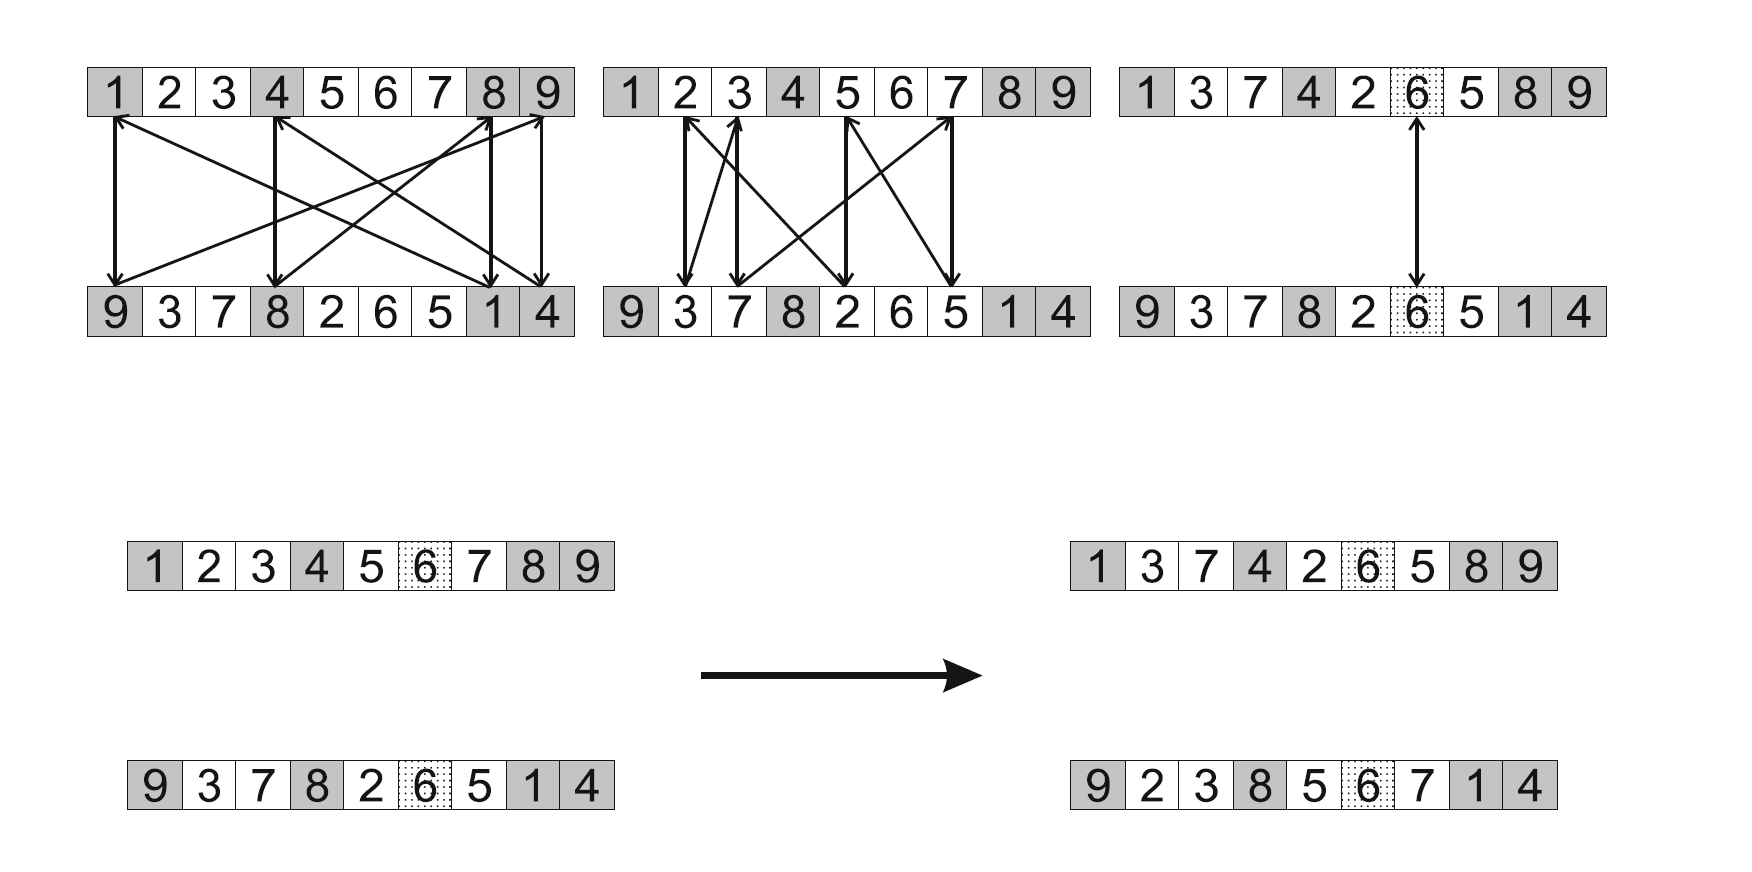
\includegraphics[width=.6\textwidth]{img/cyclecrossover.png}
  \caption{Cycle crossover \cite{EibenA.E2015ItEC}}
  \label{fig:cyclecrossover}
\end{figure}
\paragraph{DPX crossover:} This operator has been developed for the TSP in particular \cite{dpxcrossover}. This type of crossover keeps diversity by ensuring that the offspring inherits all edges common to both parents, but none of the edges that are only in one parent. This way, the generated offspring is at the same distance as its parents, hence the name distance preserving crossover. It makes use of a heuristic to join the subtours inherited from the parents. Figure~\ref{fig:dpxcrossover} shows the procedure. The tour of the first parent is copied to the offspring. After this, all edges that are not common in both parents are removed. This leaves a number of fragments consisting of one or more cities. The greedy heuristic now reconnects all edges. For each end city of a fragment, it looks for the start or end city of an other fragment such that the cost between those two are minimal. It connects these two cities if this edge is not already in one of the parents (to preserve same distance, cf. supra).
When there is little overlap between the parents, the common edges are preserved. But the offspring will be quite different because the edges that were not common in the parents will not be used again. This is beneficial because the (good) common parts of the parents are preserved, and the generated offspring is diverse. 

\begin{figure}[H]
  \centering
  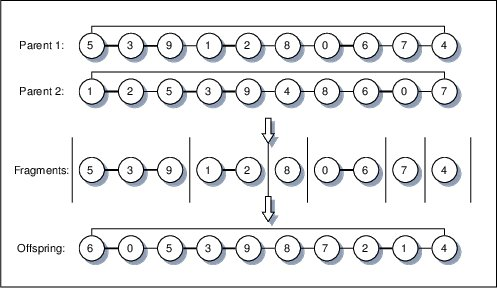
\includegraphics[width=.6\textwidth]{img/dpxcrossover.jpg}
  \caption{Illustration of the DPX crossover \cite{dpxcrossover} }
  \label{fig:dpxcrossover}
\end{figure}


\subsection{Elimination operators}\label{ssec:elimination}

% \ReplaceMe{Which elimination operators did you implement? If they are not from the slides, describe them. Why did you select this one? Are there parameters that need to be chosen? Did you use an advanced scheme to vary these parameters throughout the iterations? Did you try other elimination operators not included in the final version? Why did you discard them?}

Three elimination operators have been implemented and tested, namely ($\lambda$+$\mu$)-elimination, ($\lambda$,$\mu$)-elimination, and k-tournament elimination. The used scheme in the final code is ($\lambda$+$\mu$)-elimination because it was slightly faster than k-tournament elimination. It also gave better results than ($\lambda$,$\mu$)-elimination. Only the best individuals are promoted to the next generation, therefore it is likely to lose diversity. To counter this, a large population size of 250 individuals and crowding is used to explicitly promote diversity (See~\ref{ssec:diversitypromotion}). 

\subsection{Local search operators}\label{ssec:localsearch}

% \ReplaceMe{What local search operators did you implement? Describe them. Did they cause a significant improvement in the performance of your algorithm? Why (not)? Did you consider other local search operators that did not make the cut? Why did you discard them? Are there parameters that need to be determined in your operator? Do you use an advanced scheme to determine them (e.g., adaptive or self-adaptive)?}
Local search has been used with the initialization of the population and with the DPX operator. A part of the population is initialized with a heuristic, namely the nearest neighbour algorithm. A tour starts with a random individual, and repeatedly visits the nearest city until all have been visited. This allows the algorithm to start immediately in a promising area of the search space and speeds up the optimization process. This is needed because of the time constraint of five minutes. Nearest neighbour also has been used in DPX crossover. This is already discussed in Section~\ref{ssec:recombination}.
I also considered to implement two-opt. Two-opt avoids routes that intersect each other. The basic move behind two-opt is the same as reverse sequence mutation: it selects a part of the tour and reverses the order of this part. The difference is that two-opt keeps repeating this until improvement is made. But because I already used reverse sequence mutation, it would not have a great effect. It also comes with a high computational cost and I decided to run more iterations instead.  

\subsection{Diversity promotion mechanisms}\label{ssec:diversitypromotion}

% \ReplaceMe{Did you implement a diversity promotion scheme? If yes, which one? If no, why not? Describe the mechanism you implemented. In what sense does the mechanism improve the performance of your evolutionary algorithm? Are there parameters that need to be determined? Did you use an advanced scheme to determine them?}
In order to promote diversity, crowding has been used in combination with the elimination scheme. It works as follows: it ranks the population according to their fitness as in ($\lambda$+$\mu$)-elimination. Then the list is run through and the individual is copied each time to the next generation. Whenever this happens, a close individual is eliminated from the rest of the list. This is repeated until the population size is reached. This process is shown in Figure~\ref{fig:crowding}
The distance between individuals is determined by the number of common edges of their tours. All edges of an individual's tour are saved in an edge set after this, the intersection is made. A lot of common edges means a small distance between indentation and vice versa. 
In order to reduce computation time of crowding, the eliminated individual is determined by sampling five individuals from the population and selecting the closest one. In addition, the chance of eliminating whenever an individual is promoted ($p_{cw}$) has been set to 20\%.

\begin{figure}[H]
  \centering
  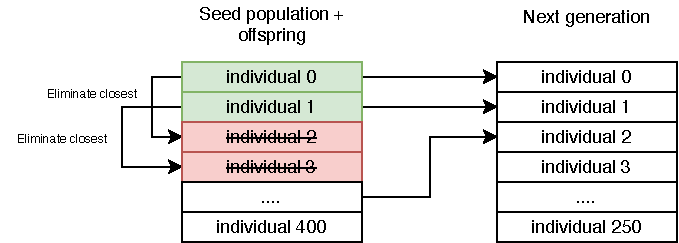
\includegraphics[width=.5\textwidth]{img/crowding.pdf}
  \caption{crowding procedure}
  \label{fig:crowding}
\end{figure}
\subsection{Stopping criterion}\label{ssec:stopcriterion}

% \ReplaceMe{Which stopping criterion did you implement? Did you combine several criteria?}
In the final code, no stopping criterion has been used. This with the aim to find the best possible solution after five minutes. A small stop criterion has been used for testing the algorithm on tour29. Every 100 iterations, it checks whether the best individual has improved. If not, the algorithm is stopped.

\subsection{The main loop}\label{ssec:mainloop}

Figure~\ref{fig:codeflow} shows the flow of the genetic algorithm. At the start, the distance matrix is checked whether there are disconnected cities. After that, the population is initialized. 75\% of the population consists of individuals with a random tour and 25\% are heuristic good individuals. Now, the optimize loop starts. Parents are picked from the population with k-tournament and create offspring with either order crossover (90\% chance) or DPX crossover (10\% chance). When this is done, one of the mutation operators is carried out to the offspring and the population. Only the best individual of the population cannot be mutated to ensure the best solution will not change. Lastly, ($\lambda$+$\mu$)-elimination with crowding (20\% chance) is used to leave a new generation of 250 individuals. 
There is no universal valid approach for the order of mutation and recombination. This order is chosen because it just works. The selection/elimination for the next generation is done by selecting the ranked individuals one by one without replacement to prevent copies of individuals in the next generation.
The choice of the parameters is described in Section~\ref{ssec:parameters}.

\begin{figure}[H]
  \centering
  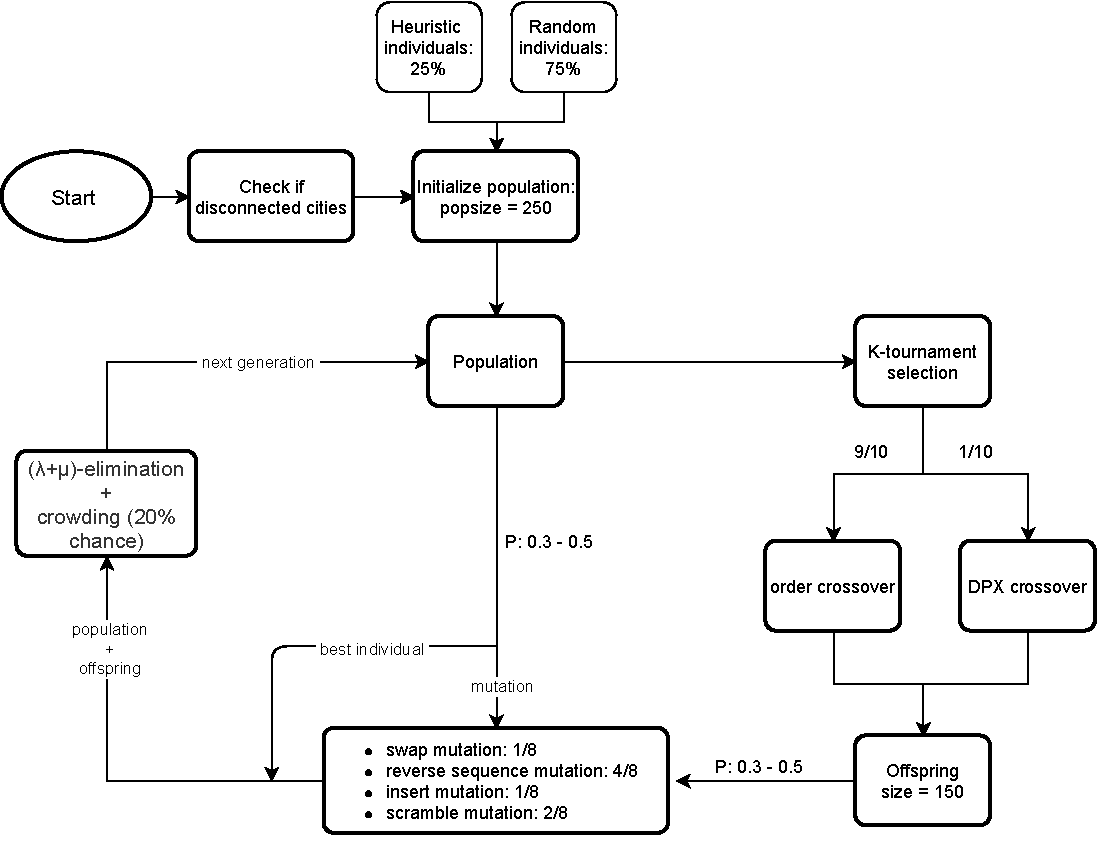
\includegraphics[width=\linewidth]{img/codeflow.pdf}
  \caption{Main loop of the algorithm}
  \label{fig:codeflow}
\end{figure}

% \ReplaceMe{Describe the main loop of your evolutionary algorithm using a clear picture (preferred) or high-level pseudocode. In what order do you apply the various operators? Why that order? If you are using several selection, mutation, recombination, elimination, and local search operators, describe how you choose among the possibilities. Are you selecting/eliminating all individuals in parallel, or one by one? With or without replacement?}

\subsection{Parameter selection}\label{ssec:parameters}

% \ReplaceMe{For all of the parameters that are not automatically determined by adaptivity or self-adaptivity (as you have described above), describe how you determined them. Did you perform a hyperparameter search? How did you do this? How did you determine these parameters would be valid both for small and large problem instances?}
The following hyperparameters are used in the algorithm:

\begin{itemize}
  \item population size: 250
  \item amount of offspring: 150
  \item k for k-tournament: 5
  \item \% heuristic individuals: 25\%
  \item probability of crowding: 15\%
  \item probability of mutation: 30-50\%
\end{itemize}
The values for the population size and k are determined in the group phase. These values turned out to give a good trade-off between their result and computation time. These values are linked because a higher population size also needs a higher selective pressure (determined by k).
The other parameters are determined by trial-and-error. This is done by adjusting the parameters stepwise after 5 runs on tour194. Then the best and variation on the best individual is checked to determine the parameter. These parameter values are also valid for the smaller problems, but are not optimal on the largest tour. The larger tour may need other values in order to run faster (e.g. smaller population size).

\subsection{Other considerations}\label{ssec:considerations}

% \ReplaceMe{Did you consider other items not listed above, such as elitism, multiobjective optimization strategies (e.g., island model, pareto front approximation), a parallel implementation, or other interesting computational optimizations (e.g. using advanced algorithms or data structures)? You can describe them here or add additional subsections as needed.}
\paragraph{Computational optimizations:} Some code optimizations have been done in order to do as many iterations as possible in the five-minute time limit. Redundant calculations of the cost of a tour and the edges of a tour (for calculating distances between individuals) are avoided by saving these values in the Individual 'object' and only recalculating them when a tour has changed. This seemed a trivial thing, but actually saves a lot of time. All parameters of the GA also have been grouped in a separate class to obtain more overview in the code. 

\paragraph{Not implemented:} Some other interesting optimizations have been considered, but not implemented because of the limited time for this project. I tried implementing the island model because I believe it may yield good results. I did not proceed with this because it completely messed up the structure in my code and I no longer had a good understanding of the code. \\

Some things like parent selection, crossover and mutation could be done in parallel. Thus, a genetic algorithm that uses multithreading in its code could provide even more gains in computation time. I did do this because it would ask too much time and I think it falls outside the scope of this course. 



\section{Numerical experiments}

% \RemoveMe{\textbf{Goal:} Based on this section and our execution of your code, we will evaluate the performance (time, quality of solutions) of your implementation and your ability to interpret and explain the results on benchmark problems.}

\subsection{Metadata}

% \ReplaceMe{What parameters are there to choose in your evolutionary algorithm? Which fixed parameter values did you use for all experiments below? If some parameters are determined based on information from the problem instance (e.g., number of cities), also report their specific values for the problems below.

% Report the main characteristics of the computer system on which you ran your evolutionary algorithm. Include the processor or CPU (including the number of cores and clock speed), the amount of main memory, and the version of Python 3.}
The parameters that were used for the evolutionary algorithm are listed below. Most of them are fixed. Only the alpha value changes over time but stays within the range of 0.3-0.5.
\begin{itemize}
    \item population size $\lambda$: 250
    \item \% initialized with heuristic individuals: 25\%
    \item amount of offspring $\mu$: 150
    \item k-tournament k: 5
    \item mutation probability $\alpha$: 0.3-0.5
    \item recombination probability $p_{rc}$: 0.99
\end{itemize}
Specifications of the computer system used for the experiments:
\begin{itemize}
    \item CPU: Intel Core i7-8550, 4 cores @1.80 GHz (code is not adapted for multi-threading)
    \item 8 GB main memory
    \item Python version 3.8
\end{itemize}


\subsection{tour29.csv}

% \ReplaceMe{Run your algorithm on this benchmark problem (with the 5 minute time limit from the Reporter). Include a typical convergence graph, by plotting the mean and best objective values in function of the time (for example based on the output of the Reporter class). 

% What is the best tour length you found? What is the corresponding sequence of cities? 

% Interpret your results. How do you rate the performance of your algorithm (time, memory, speed of convergence, diversity of population, quality of the best solution, etc)? Is your solution close to the optimal one?

% Solve this problem 1000 times and record the results. Make a histogram of the final mean fitnessess and the final best fitnesses of the 1000 runs. Comment on this figure: is there a lot of variability in the results,    what are the means and the standard deviations?}

The best tour length found for this problem was $27154.49$. This seems to be the optimal solution for this problem. The corresponding sequence of cities of this tour is: 
\begin{align*}
    \text{[ 5  0  1  4  7  3  2  6  8 12 13 15 23 24 26 19 25 27 28 22 21 20 16 17 18 14 11 10  9] }
\end{align*}
A typical convergence graph is shown in Figure~\ref{fig:convergence}. For this benchmark problem, a simple stop criterion has been used to speed up the experiment. Every 100 iterations the algorithm checks if there is any improvement. If there is not, the optimization process is stopped. The average time to find the optimal solution is around five seconds. The algorithm does perform very well for this small problem. It mostly finds the optimal solution in a short period. The diversity in the population is high enough until it finds the optimal solution. 
\begin{figure}[H]
    \centering
    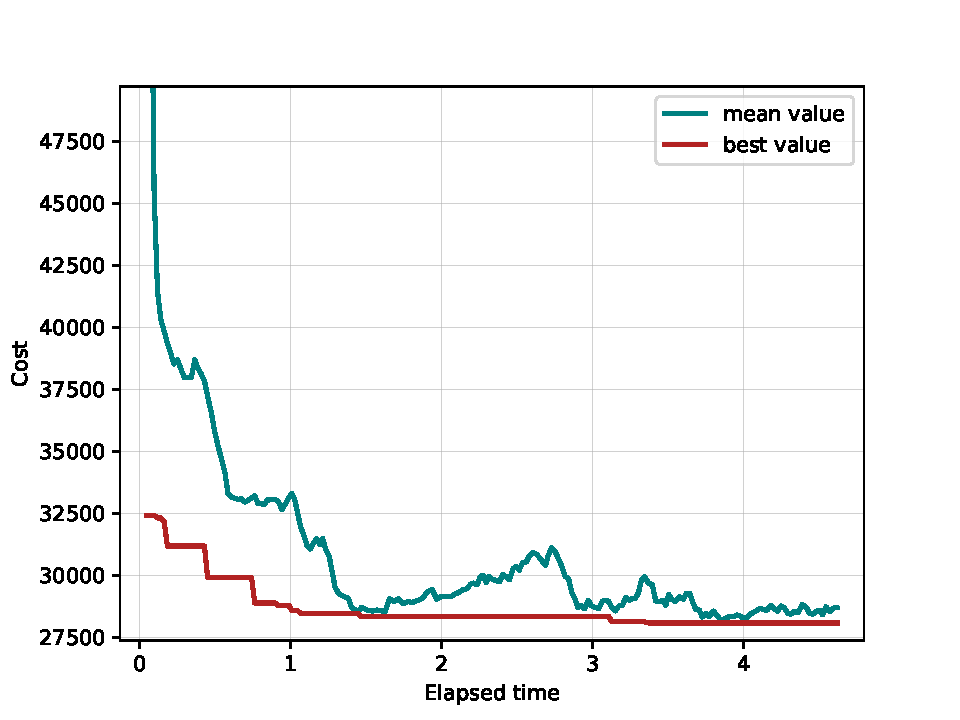
\includegraphics[width=.8\linewidth]{img/convergence.pdf}
    \caption{Typical convergence graph of tour29.csv}
    \label{fig:convergence}
\end{figure}
Figure~\ref{fig:variations} shows the histograms that are obtained when running the problem 1000 times with the GA. It can be seen that the algorithm finds the optimal solution in 3/4 cases. Sometimes it stops with a not-optimal value that is close to the optimal one. From Figure~\ref{fig:variationmean}, it can be seen that the cost of the mean population usually is quite higher. There may be a little more exploitation needed at the end of the algorithm in order to lower the average cost of the population and to find the optimal solution every time. Now, the algorithm often gets stuck in a local optimum of $\pm 28300$. Nevertheless, without a stop criterion the algorithm always finds the optimal value within 5 minutes.
\begin{figure}[H]
    \begin{subfigure}{0.55\linewidth}
      \centering
      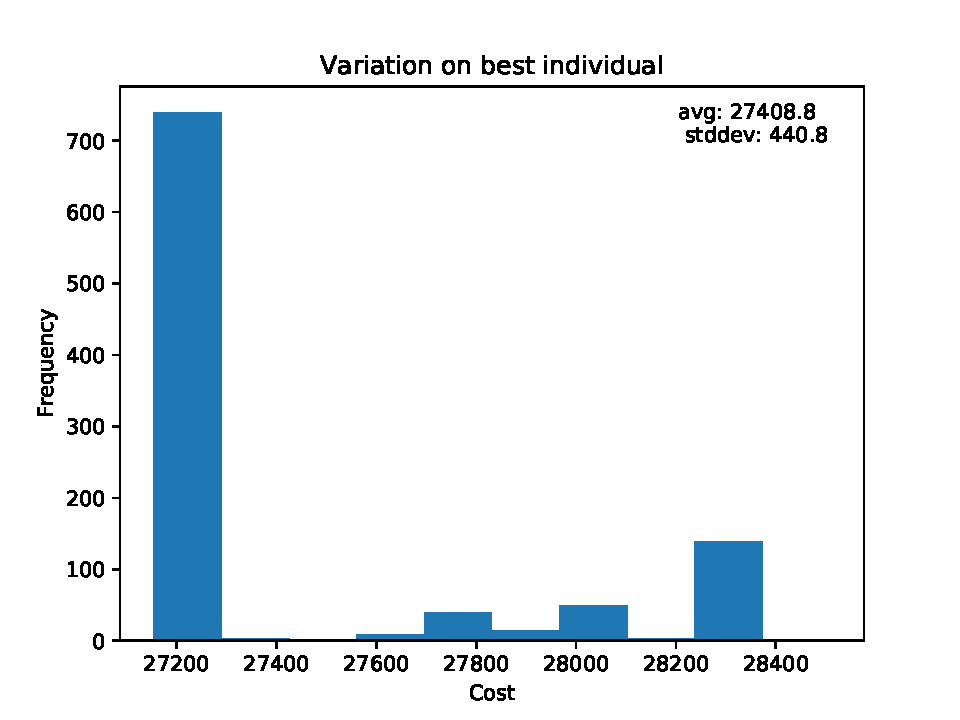
\includegraphics[width=\linewidth]{img/variationbest.pdf}
      \caption{variation on the best individual}
      \label{fig:variationbest}
    \end{subfigure}
    \begin{subfigure}{0.5\linewidth}
      \centering
      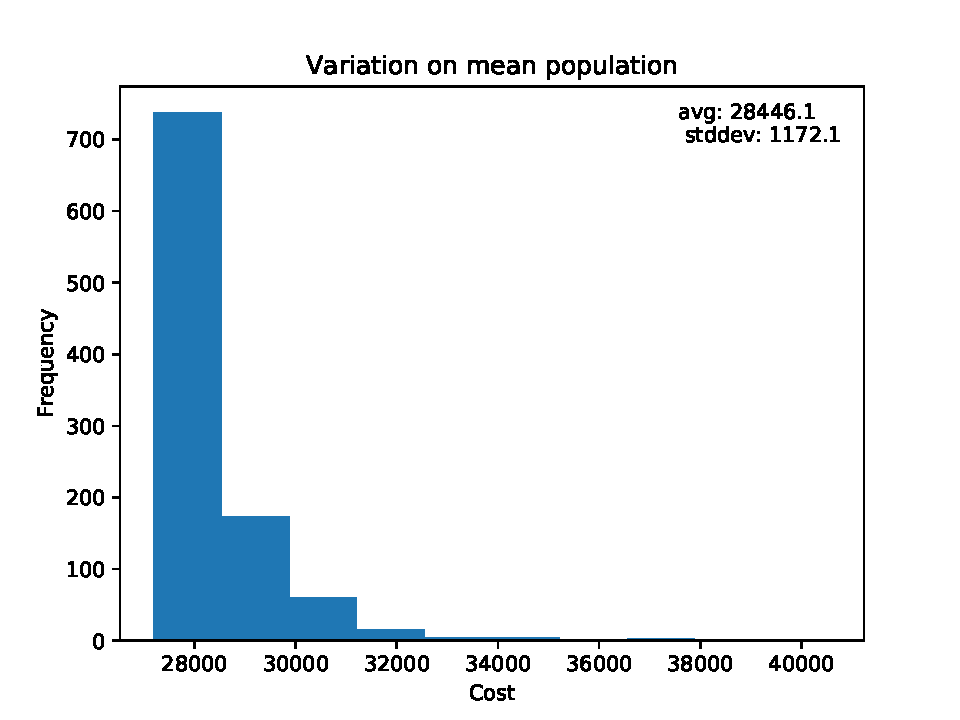
\includegraphics[width=\linewidth]{img/variationmean2.pdf}
      \caption{variation on the mean individual}
      \label{fig:variationmean}
    \end{subfigure}
    \caption{Histograms that shows the variation on the best individual and mean individual when the problem is run 1000 times}
    \label{fig:variations}
  \end{figure}

\subsection{tour100.csv}
A typical convergence graph of this problem is shown in Figure~\ref{fig:convergence100}. It can be seen that the algorithm converges too quickly after \SI{50}{\second}. At this point, the algorithm does not find a better solution and start searching in a wrong direction (hence the increase in mean cost). The spikes on the mean cost are due to tours with disconnected cities. The cost of these tours has been set very high, which causes the spikes in the mean population.

The lowest cost that has been found with this algorithm is 7521. This is better than the heuristic value of 8637, but still 200 higher than the optimal value of around 7350. The hyperparameters are probably not optimal for this problem.
\begin{figure}[H]
  \centering
  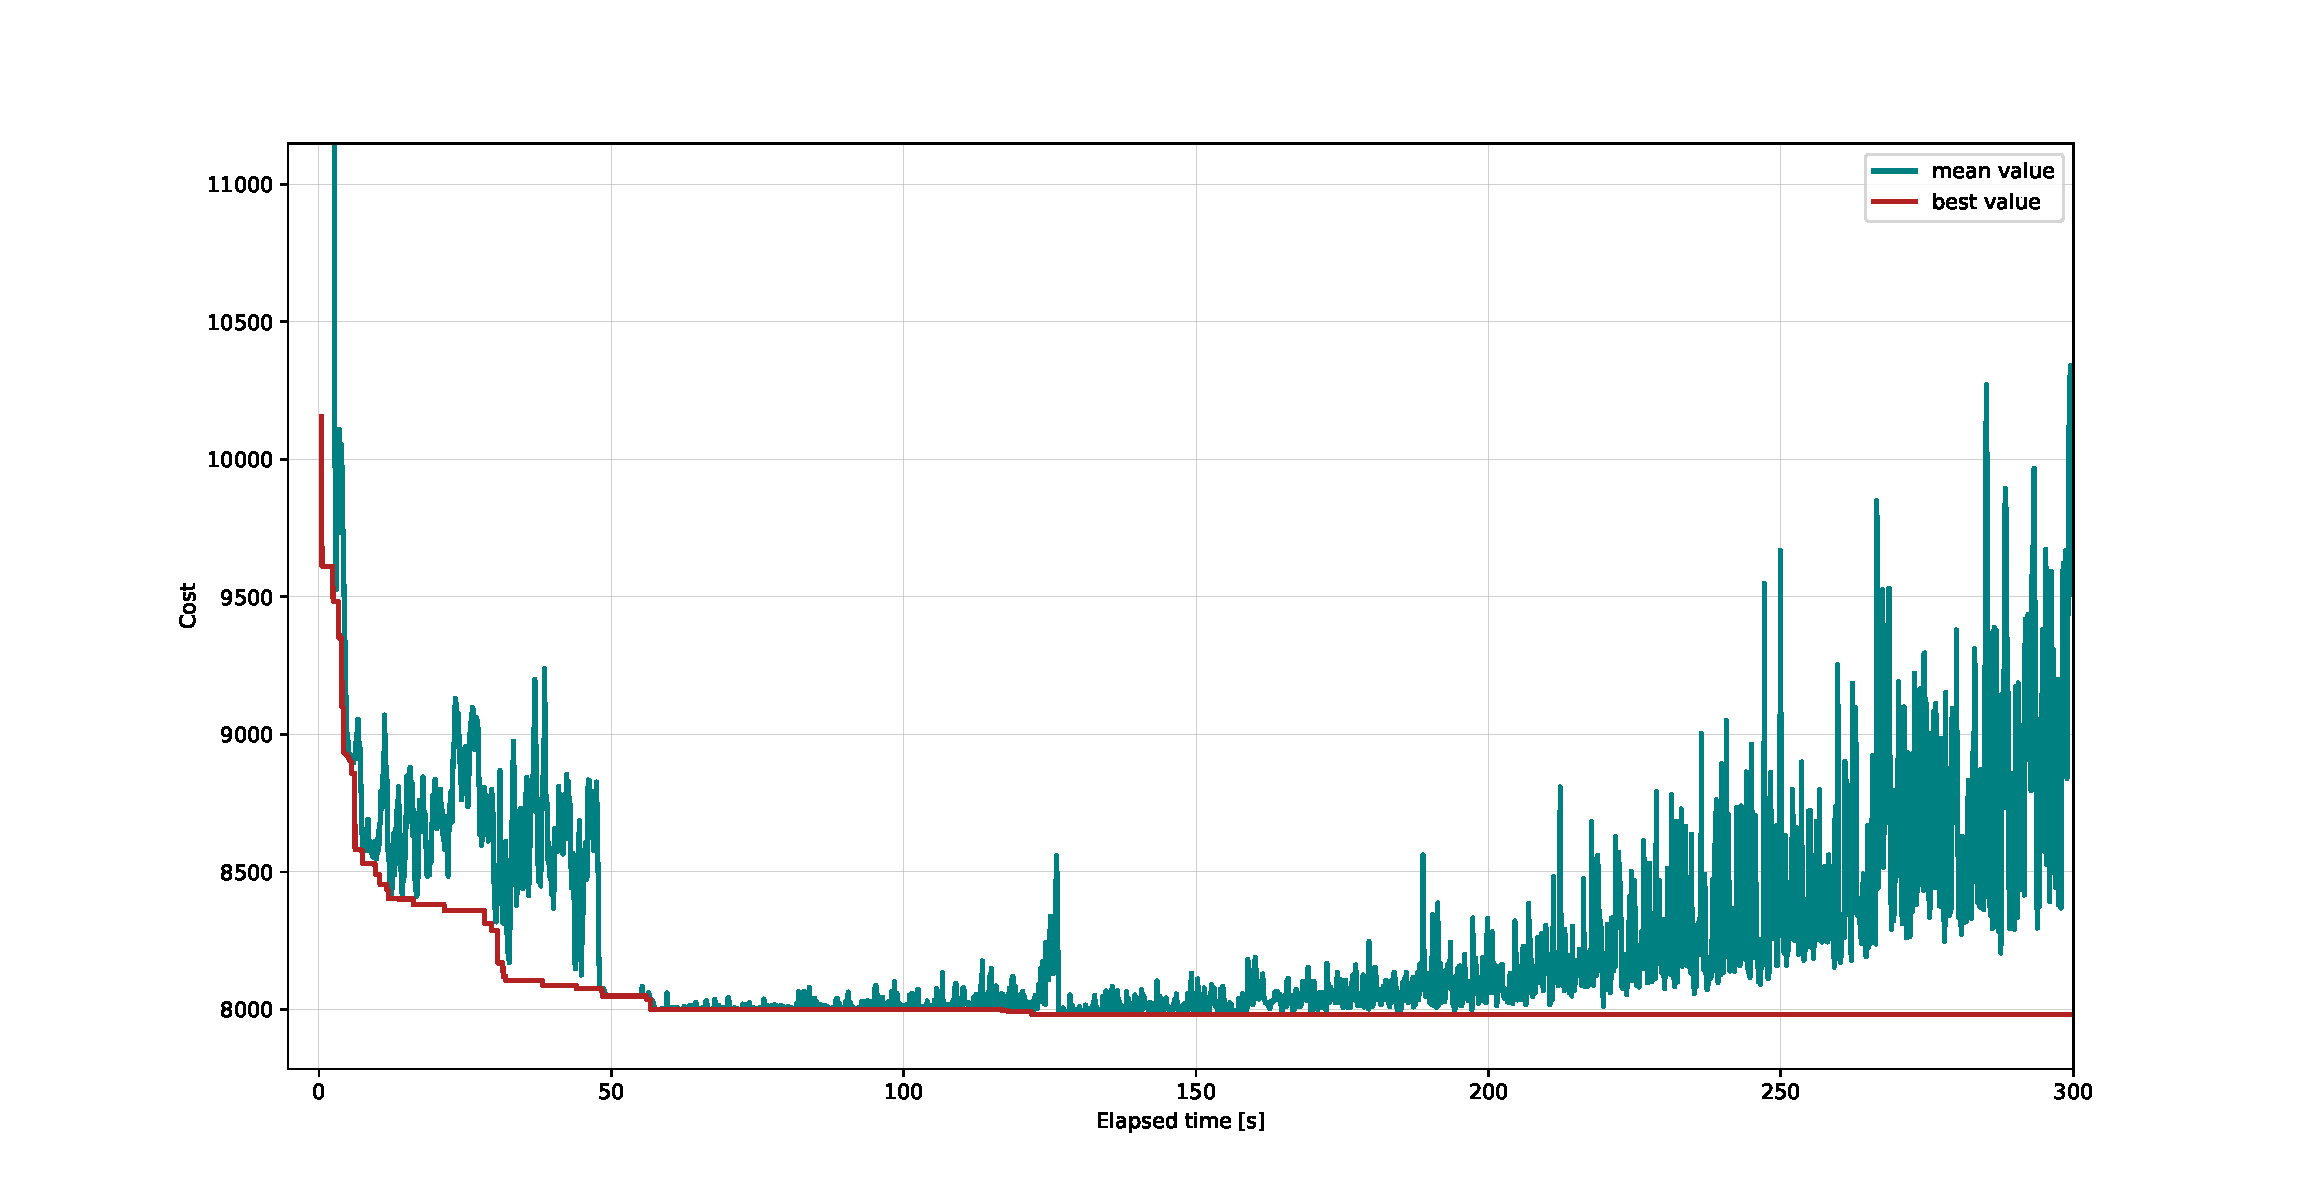
\includegraphics[width=.8\linewidth]{img/convergence100.pdf}
  \caption{Convergence graph tour100}
  \label{fig:convergence100}
\end{figure}

% \ReplaceMe{Run your algorithm on this benchmark problem (with the 5 minute time limit from the Reporter). Include a typical convergence graph, by plotting the mean and best objective values in function of the time (for example based on the output of the Reporter class). 

% What is the best tour length you found in each case? 

% Interpret your results. How do you rate the performance of your algorithm (time, memory, speed of convergence, diversity of population, quality of the best solution, etc)? Is your solution close to the optimal one?}


\subsection{tour194.csv}

% \ReplaceMe{Run your algorithm on this benchmark problem (with the 5 minute time limit from the Reporter). Include a typical convergence graph, by plotting the mean and best objective values in function of the time (for example based on the output of the Reporter class). 

% What is the best tour length you found? 

% Interpret your results. How do you rate the performance of your algorithm (time, memory, speed of convergence, diversity of population, quality of the best solution, etc)? Is your solution close to the optimal one?}
Figure~\ref{fig:convergence194} shows a typical convergence graph. The best-found tour length is 9843. The diversity here is good, as the mean cost always is a bit higher than the best cost. The algorithm finds in 5 minutes a value that is clearly better than the heuristic value (11385). The optimal value is 800 less, so the algorithm still can be improved to find a better solution in five minutes. 
\begin{figure}[H]
  \centering
  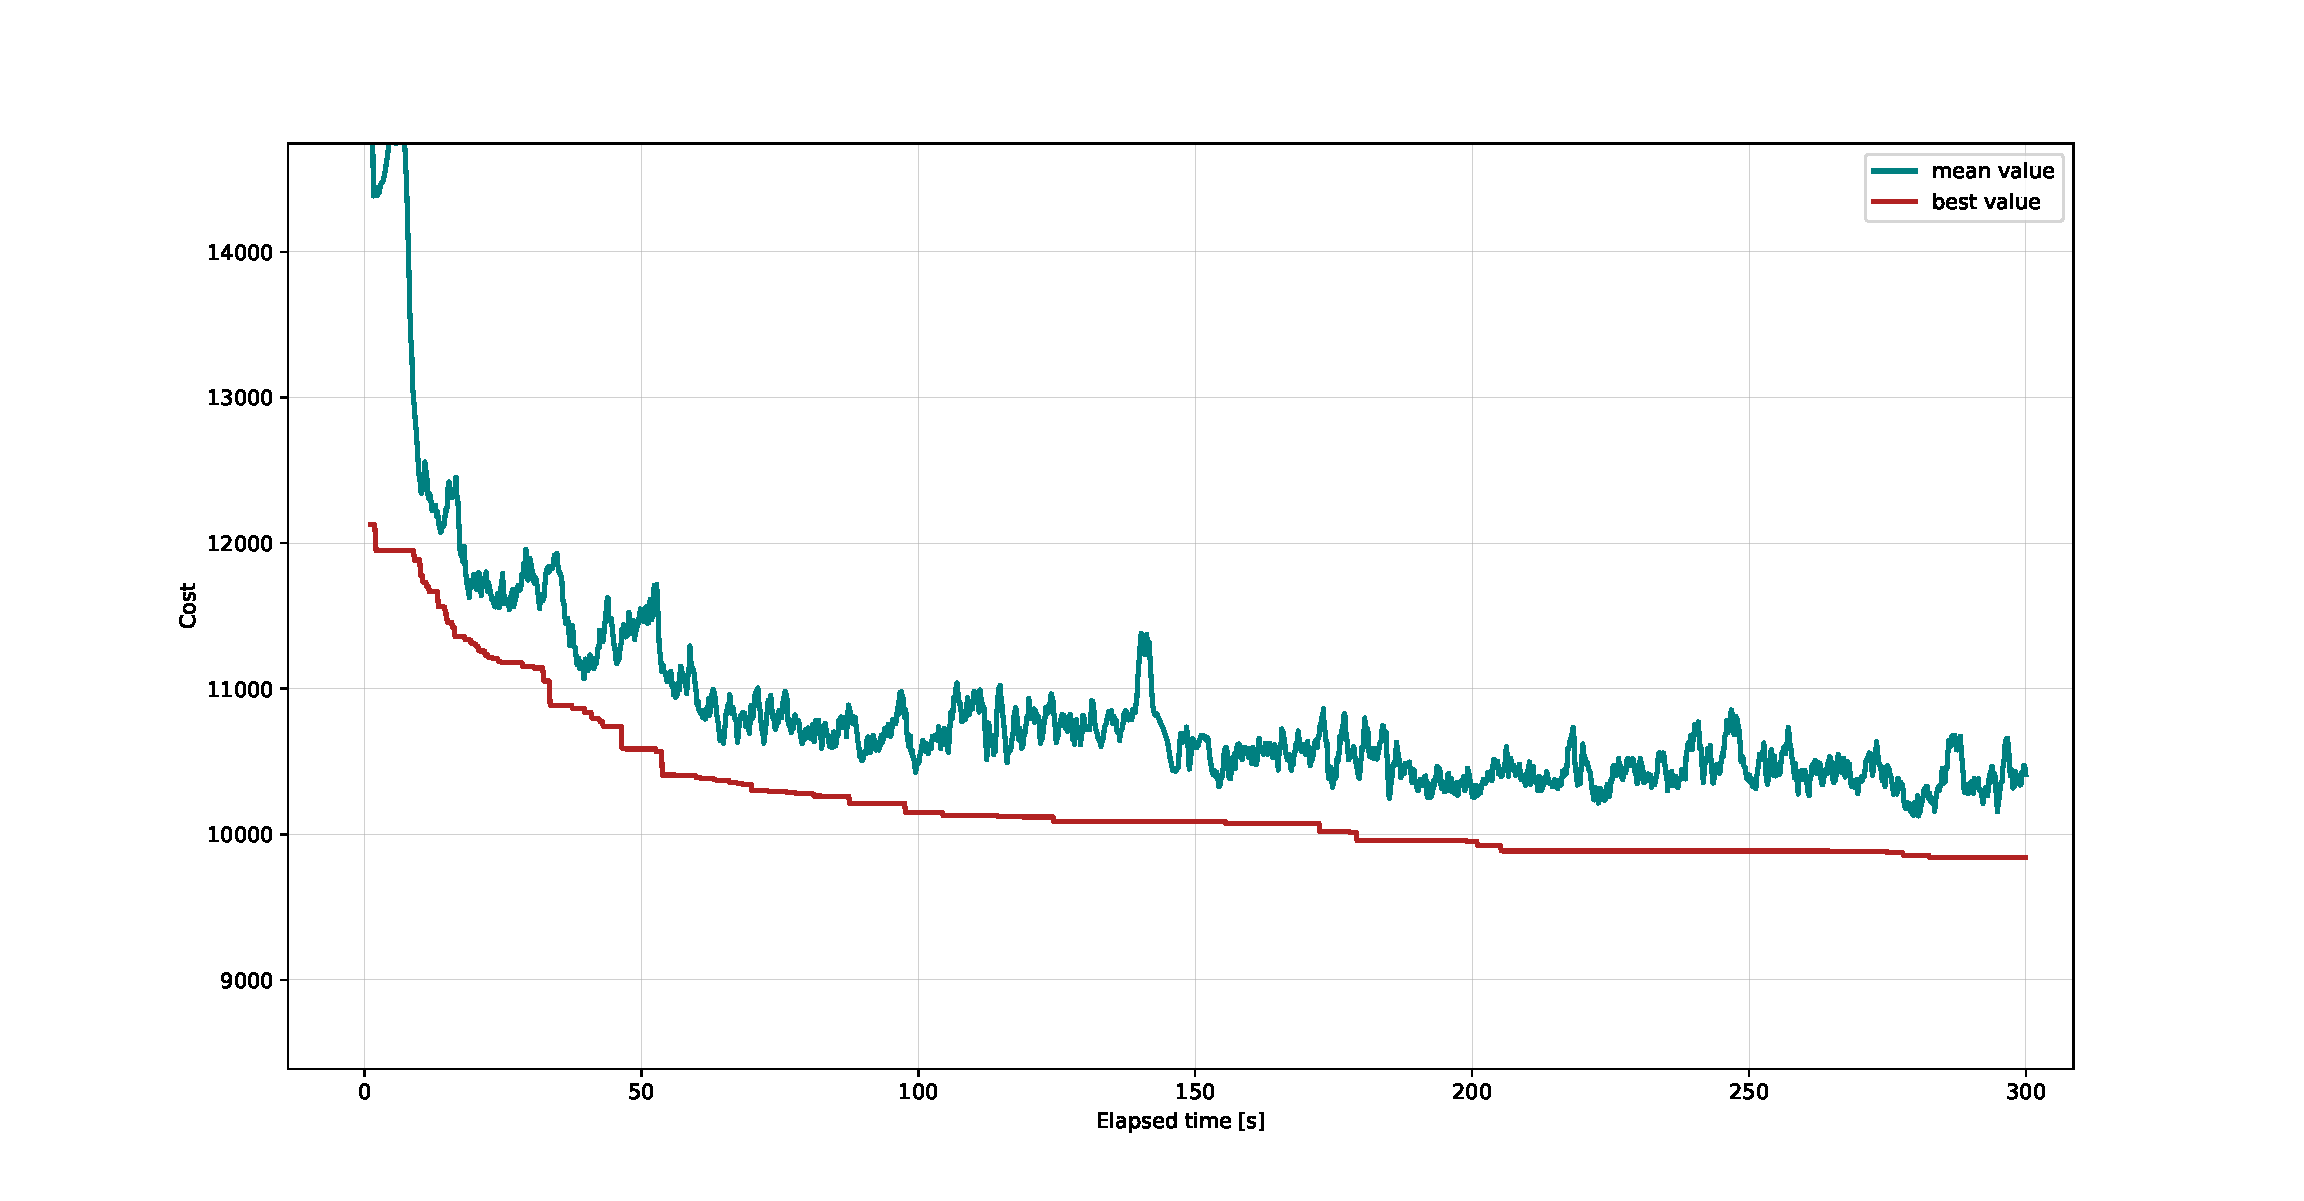
\includegraphics[width=.8\linewidth]{img/convergence194.pdf}
  \caption{Convergence graph tour194}
  \label{fig:convergence194}
\end{figure}

\subsection{tour929.csv}
Figure~\ref{fig:convergence194} shows a typical convergence graph. The best-found tour has a cost of 112205. This is slightly better than the heuristic value (113683). However, the optimal value of 95300 is still far away. The algorithm does not perform well on bigger tours because the parameters are not optimized. The diversity is too high and the algorithm does not converge to an optimal value. The algorithm is too explorative here. Also, the algorithm is a lot slower on these bigger tours and less iterations can be done in five minutes. 
\begin{figure}[H]
  \centering
  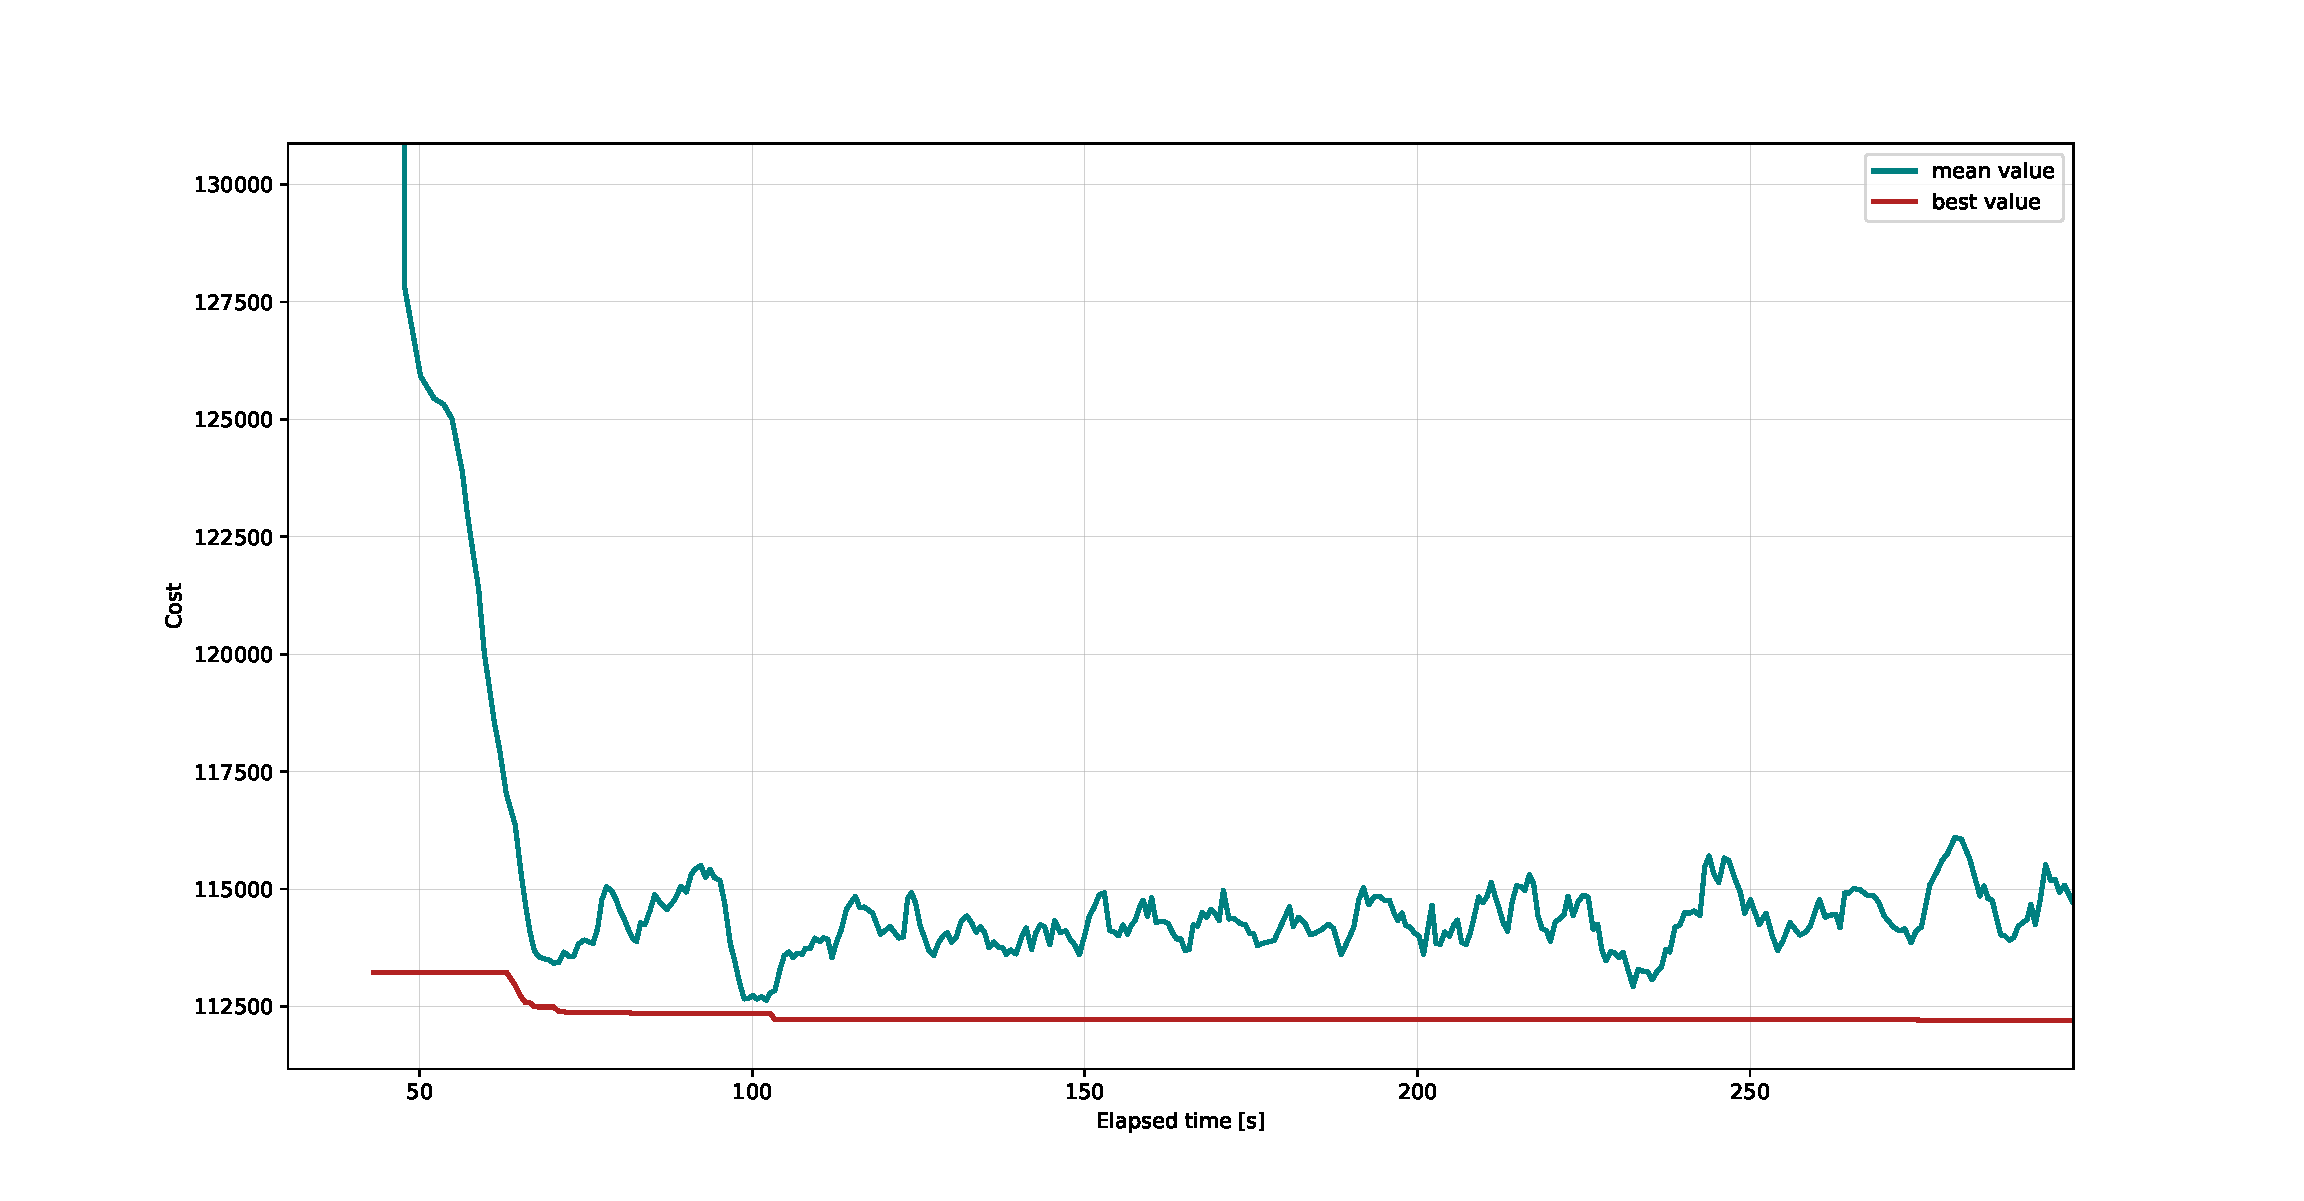
\includegraphics[width=.8\linewidth]{img/convergence929.pdf}
  \caption{Convergence graph tour929}
  \label{fig:convergence929}
\end{figure}.

% \ReplaceMe{Run your algorithm on this benchmark problem (with the 5 minute time limit from the Reporter). Include a typical convergence graph, by plotting the mean and best objective values in function of the time (for example based on the output of the Reporter class). 

% What is the best tour length you found? 

% Interpret your results. How do you rate the performance of your algorithm (time, memory, speed of convergence, diversity of population, quality of the best solution, etc)? Is your solution close to the optimal one? 

% Did your algorithm converge before the time limit? How many iterations did you perform?}



\section{Critical reflection}

% \RemoveMe{\textbf{Goal:} Based on this section, we will evaluate your understanding and insight into the main strengths and weaknesses of your evolutionary algorithms.}

% \ReplaceMe{Describe the main lessons learned from this project. What do you think are the main strong points of evolutionary algorithms in general? Did you apply these strengths in this project? What are the main weaknesses of evolutionary algorithms and of your implementation in particular? Do you think these can be avoided or mitigated? How? Do you believe evolutionary algorithms are appropriate for this problem? Why (not)? What surprised you and why? What did you learn from this project?}
The main strengths of a GA are in my opinion that it can be used in various representations and thus problems. It can come up relatively fast with good solutions and the basic concept is easy to understand. In my algorithm, I also tried to optimize the code such it can run iterations fast and come up with good solutions for this problem in a short period.
I think the main weakness of a GA is the tuning of the different parameters. This is also the main weakness in my algorithm. There are a lot of parameters to be considered (k in k-tournament, $\alpha$ for mutation, $\lambda$ for population size, $\mu$ for amount of offspring, \ldots). The parameters are chosen based on tour194 but may be not the best for the others. It is time-consuming and sometimes difficult to find out what the best values for these parameters are. One can try to implement self-adaptivity, where the different parameters adapt with every new generation. But there is no 'one size fits all' solution and self-adaptivity is still subject of many studies today.  \\

An evolutionary algorithm is very appropriate for the TSP in my opinion. A brute force approach would be way too slow because of the very high number of possible tours. The algorithm can also build on existing heuristics for this problem to come up with even better solutions. \\

I thought it was cool that this course is very hands-on. It did certainly improve my python programming skills. Before I did not know about the existence of GA's and now, I am able to set up a (basic) genetic algorithm. The drawback is that the study load of this course was quite high during the semester.



% \section{Other comments} \label{sec_other}

% \ReplaceMe{In case you think there is something important to discuss that is not covered by the previous sections, you can do it here. }

\bibliography{bibliography}
\bibliographystyle{ieeetr}

\end{document}
